\begin{picture}(440,275)
		\put(0,0){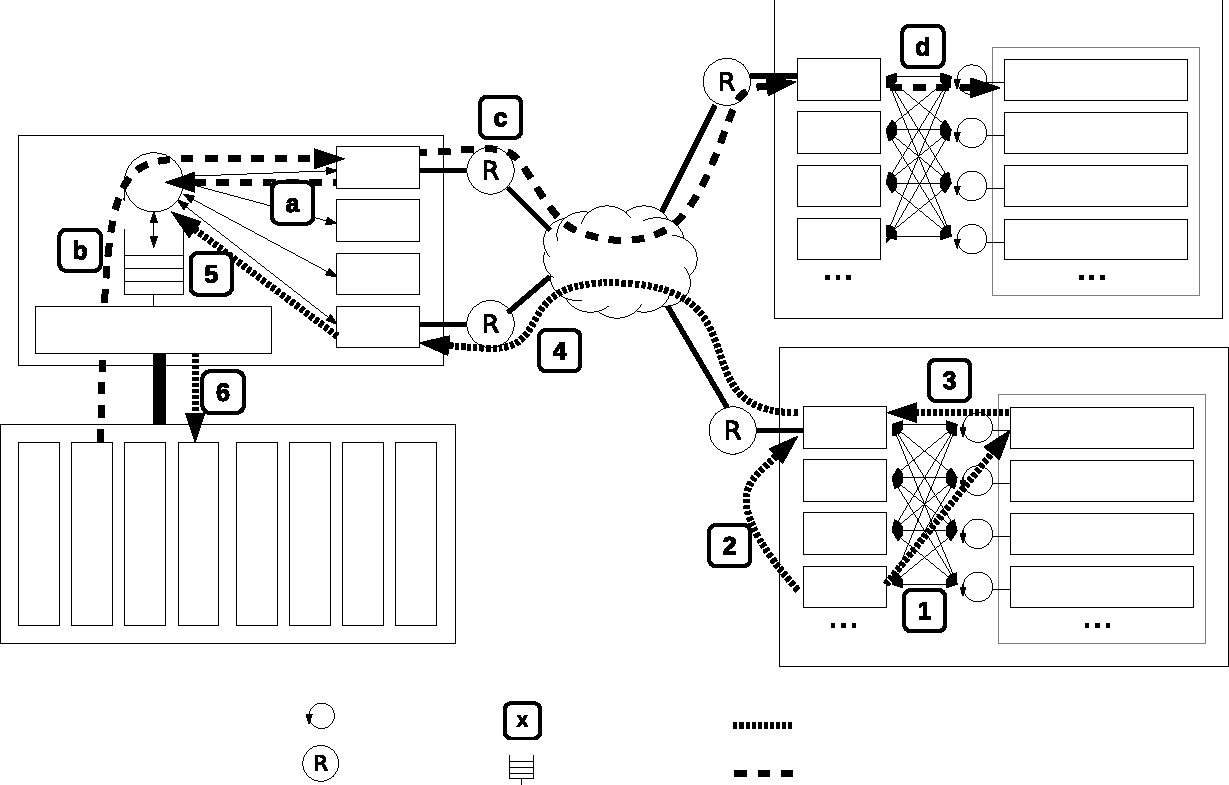
\includegraphics[width=15cm]{imgs/pdf/systemModel_MPPAremoteMem.pdf}}
		\put(371,65){\scriptsize Banc 4}
		\put(371,83){\scriptsize Banc 3}
		\put(371,102){\scriptsize Banc 2}
		\put(371,120){\scriptsize Banc 1}
		\put(368,186){\scriptsize Banc 4}
		\put(368,204){\scriptsize Banc 3}
		\put(368,223){\scriptsize Banc 2}
		\put(368,241){\scriptsize Banc 1}
		\put(355,140){\footnotesize SRAM Locale}
		\put(355,260){\footnotesize SRAM Locale}
		\put(429,146){\rotatebox{270}{\footnotesize Cluster B}}
		\put(427,267){\rotatebox{270}{\footnotesize Cluster A}}
		\put(282,65){\scriptsize C\oe{}ur 3}
		\put(282,83){\scriptsize C\oe{}ur 2}
		\put(282,102){\scriptsize C\oe{}ur 1}
		\put(284,120){\scriptsize DMA}
		\put(279,186){\scriptsize C\oe{}ur 3}
		\put(279,204){\scriptsize C\oe{}ur 2}
		\put(279,223){\scriptsize C\oe{}ur 1}
		\put(282,241){\scriptsize DMA}
		\put(206,179){\footnotesize NoC}
		\put(119,211){\scriptsize DMA 1}
		\put(120,193){\scriptsize C\oe{}ur 2}
		\put(120,175){\scriptsize C\oe{}ur 1}
		\put(119,156){\scriptsize DMA 2}
		\put(23,155){\footnotesize Contrôleur DDR}
		\put(95,127){\footnotesize DDR-SDRAM}
		\put(100,227){\footnotesize Cluster IO}
		\put(10,75){\rotatebox{90}{\scriptsize Banc 1}}
		\put(30,75){\rotatebox{90}{\scriptsize Banc 2}}
		\put(48,75){\rotatebox{90}{\scriptsize Banc 3}}
		\put(66,75){\rotatebox{90}{\scriptsize Banc 4}}
		\put(86,75){\rotatebox{90}{\scriptsize Banc 5}}
		\put(104,75){\rotatebox{90}{\scriptsize Banc 6}}
		\put(123,75){\rotatebox{90}{\scriptsize Banc 7}}
		\put(141,75){\rotatebox{90}{\scriptsize Banc 8}}
		\put(122,21){\footnotesize Arbitre}
		\put(122,5){\footnotesize Routeur Noc}
		\put(194,20){\footnotesize Étape}
		\put(194,5){\footnotesize File d'attente}
		\put(282,18){\footnotesize Procédure d'écriture}
		\put(282,4){\footnotesize Procédure de lecture}
	\end{picture}
